\chapter[Metodologia]{Metodologia}
\label{metodologia}
Nesse capítulo são apresentadas a medida de correlação utilizada no trabalho, além das principais características do \textit{framework}, mostrando como a correlação é aplicada
para a detecção de ataques DDoS e quais bases de dados são utilizadas para a avaliação do \textit{framework}, destacando sua estrutura e ferramentas utilizadas para o tratamento dos dados.
% ----------------------------------------------------------

\section{Modelo de correlação NaHiD}

Neste trabalho, o \textit{framework} utilizado baseia-se na correlação proposta por \cite{HOQUE201748} chamada NaHiD (nome que possivelmente provém a partir das iniciais de cada autor), cujo objetivo é distinguir objetos de tráfego normais e maliciosos. Tal medida leva em consideração principalmente o desvio padrão e a média de cada objeto, ponderando cada elemento como mostrado na equação a seguir:  

\begin{equation}
	NaHiD(X,Y) = 1 - \frac{1}{n} \sum_{i=1}^{n} \frac{\left(|X(i) -	 Y(i)|\right)}{||\mu{X} - sX| - X(i)| + ||\mu{Y} - sY| - Y(i)|}
\end{equation}
onde
\begin{itemize}
	\item $\mu{X}$: Média aritmética do objeto de tráfego X.
 	\item $\mu{X}$: Média aritmética do objeto de tráfego Y.
	\item $sX$: Desvio padrão do objeto de tráfego X.
	\item $sY$: Desvio Padrão do objeto de tráfego Y.
\end{itemize}
As provas de simetria e identidade da correlação podem ser encontradas em \cite{HOQUE201748}.

\section{Framework de detecção de ataques DDoS}
 
 \begin{figure}[ht]
	\centering
	\caption{Estrutura do \textit{framework} analisado }
	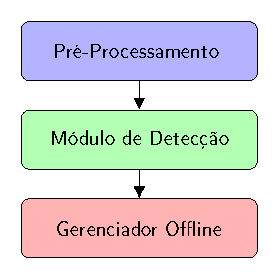
\includegraphics[width=0.5\textwidth]{figs/fluxoFramework.pdf}\\
	{Fonte: Elaborada pelo autor.}
	\label{fig:Fluxo_Framework}
\end{figure}

O \textit{framework} tem como objetivo, detectar ataques DDoS em tempo real na rede monitorada, a partir de dados trafegados na rede com uma taxa aceitável de erros. Tal arcabouço possui três módulos: pré-processamento, detecção e um de segurança. A \figref{fig:Fluxo_Framework} mostra o fluxo de funcionamento do \textit{framework}. Amostras de tráfego são capturadas de uma porta do roteador na forma de um pacote TCP/IP e enviadas ao módulo de pré-processamento. Nessa fase, a cada segundo, os pacotes recebidos são agrupados e essa instância de tráfego é enviada para o módulo de detecção de ataques, que irá classificar a instância como normal ou maliciosa. O gerente de segurança manterá um perfil normal, como referência, e um valor limiar de correlação em sua base de perfis, para ser usado pelo módulo de detecção. Incrementalmente, o gerente recalcula o perfil normal baseado nos valores anteriores. 

\subsection{Pré-Processamento}
Nessa etapa, os dados são coletados por um \textit{sniffer} da rede, o qual analisa todos os pacotes trafegados e, a cada segundo, as métricas desejadas são calculadas para servirem de entrada para a correlação NaHiD. 
\subsubsection{Entropia de IPs origem}
A entropia de IPs origem é uma medida do grau de desordem, onde ela é máxima caso todos os elementos sejam diferentes e o tamanho da entrada seja máximo, e será mínima (igual a 0) quando todos os elementos forem iguais, independentemente do tamanho. Assim, a entropia é dada pela seguinte fórmula:
\begin{equation}
H(X) = - \sum_{i}^{n}p(x_i)log_2(x_i)
\end{equation}
Onde $X$ é a entrada e representa os IPs origem das requisições e $n$ é o número total de valores possíveis para o IP origem. 
A \tabref{Tab:entropia} mostra exemplos com valores de entrada para entropia, bem como o resultado do cálculo da função.
\\
\begin{table}[!htb]
	\centering
	\begin{threeparttable}
		\caption{Exemplo de IPs origem com respectivos valores de entropia}
		\label{Tab:entropia}
		  \begin{tabular}{cccccc}
			\hline
			\multicolumn{5}{c}{IPs origem} %%\\               %% <-- mistake
			&                                            %% <--  addition
			\multicolumn{1}{|c|}{Entropia} \\\hline           %% <--  Changed
			192.168.8.8 & 192.168.8.8 & 192.168.8.8 & 192.168.8.8 & 192.168.8.8 & 0        \\
			192.168.15.129 & 192.168.8.5 & 192.168.8.8 & 192.168.10.16 & 192.168.20.22 & 2.3219\\
			192.168.8.8 & 192.168.8.8 & 192.168.8.5 & 192.168.10.16 & 192.168.20.22 & 1.9219\\
			192.168.20.22 & 192.168.20.22 & 192.168.20.22 & 192.168.20.22 & 192.168.8.8 & 0.7219\\
			\hline
		\end{tabular}
		{Fonte: Elaborada pelo autor.}
	\end{threeparttable}
\end{table}
Note que a entropia é mínima quando todos os IPs origem são iguais (primeira linha da tabela) e máxima quando todos os os IPs origem são diferentes (segunda linha). 

\subsubsection{Variação de IPs Origem}
Essa medida, diferentemente da entropia, trata-se da taxa de mudança dos IPs origem e é calculada da seguinte forma:
\begin{equation}
	V_{Ip}(X) = \frac{\delta}{N}
\end{equation}
Onde $\delta$ é o número de mudanças de IPs origem e $N$ é o numero total de IPs de entrada. Neste trabalho consideramos uma variação cada troca de valores como no exemplo:
\begin{equation}
	X = {1,2,1,2,3}
\end{equation}
Assim, nesse vetor consideram-se 4 variações ainda que sejam para um valor que repetiu-se. Assim se os IPs origem mudarem frequentemente, a variação será alta. \cite{HOQUE201748}
\\
A observação do comportamento de ataques por \textit{flood} mostra que esse tipo de ameaça pode ser gerada por atacantes reais como zumbis. Se endereços de IP origem falsificados forem utilizados durante um ataque DDoS TCP SYN, a entropia e variação de IPs origem serão altas e esse comportamento também ocorre em um tráfego normal. \cite{HOQUE201748}. Assim faz-se necessário o uso da taxa de pacotes em bits como terceiro parâmetro de entrada para o módulo de detecção.

\subsection{Módulo de Detecção}
O modulo de detecção consiste na aplicação da correlação NaHiD, utilizando os três parâmetros de entrada fornecidos pelo módulo de pré-processamento:
\begin{itemize}
	\item Variação de IPs origem
	\item Entropia de IPs origem
	\item Taxa de pacotes
\end{itemize}
Por tratar-se de uma medida de correlação é necessário manter um valor de referência para o cálculo. Assim, os parâmetros(Variação e entropia de IPs origem, além da taxa de pacotes) de um tráfego normal devem ser fixados para a comparação com a instância de tráfego a ser analisada. Além disso, define-se um limiar do resultado da correlação para distinguir instâncias normais de maliciosas. Caso a correlação calculada seja menor que esse limiar, tal tráfego em analisado não tem semelhança suficiente com o perfil normal comparado, sendo considerado um ataque.
\subsection{Gerenciador Offline}
Nessa módulo, os valores de correlação, IPs origem, destino, taxas de pacotes, além dos resultados do módulo de detecção são salvos para a janela de tráfego em análise e se o módulo de detecção identificar que o tráfego em questão é normal, este será atualizado com os valores do mesmo para a próxima janela.

\section{Aplicação do \textit{framework} de detecção em bases de dados reais}
\label{Sec:NaHiD_VERC}
Para a avaliação do trabalho, duas bases de tráfegos de rede foram escolhidas: DARPA e  DataMining[escolher melhor esse nome] os quais são mais detalhados a seguir 
\subsection{DARPA - MIT}
 A base de dados DARPA foi produzida por pesquisadores do \textit{Lincoln Laboratory} do Instituto de Tecnologia de Massachusetts nos Estados Unidos e tem por objetivo coletar dados de tráfego de rede da Força Aérea do país para encontrar vulnerabilidades em seu sistema bem como ser utilizado para avaliações futuras. Os dados foram coletados e passaram por uma fase de treinamento de 7 semanas com 38 tipos de ataques para simular ameaças internas a rede. O ambiente de rede era composto por duas partes: a rede interna da Força aérea e a rede externa que representava a Internet; ambos conectados por meio de um roteador como mostra a \figref{fig:DARPA_Estrututra}.	Assim, um \textit{sniffer} de rede foi instalado no roteador e todas as requisições para os computadores da Força aérea foram capturadas em um arquivo tcpdump, o qual pode ser encontrado em \cite{siteDarpa}. 
 \begin{figure}[ht]
 	\centering
	\caption{Estrutura de rede Base Aérea dos EUA }
		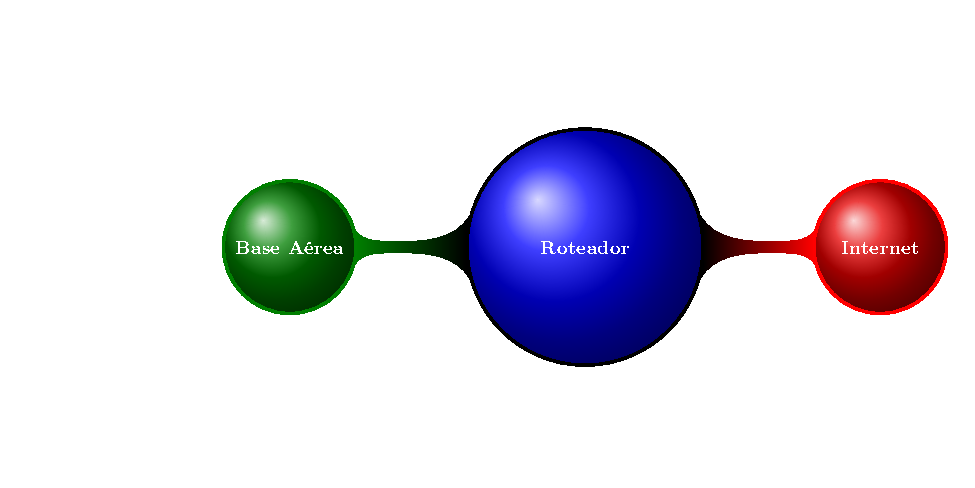
\includegraphics[width=0.8\textwidth]{figs/darpaStructure.pdf}\\
	{Fonte: Elaborada pelo autor.}
	\label{fig:DARPA_Estrututra}
\end{figure}
\\
A partir desse \textit{dataset} é possível extrair informações acerca de cada pacote transmitido durante o período de aquisição dos dados como mostra o exemplo na \tabref{Tab:WiresharkEx}.

\begin{table}[!htb]
	\centering
	\begin{threeparttable}
		\caption{Exemplo base de dados DARPA}
		\label{Tab:WiresharkEx}
		%	\small
		\begin{tabular}{c c c c c c}
			\toprule
			\textbf{Número} & \textbf{Tempo} & \textbf{Origem} & \textbf{Destino}  & \textbf{Protocolo} & \textbf{Tamanho}[bytes]
			\\ \midrule
			1 &  18:56:12.1386 &  192.168.0.20 & 192.168.0.30 & TCP & 60  \\ \midrule
			2 &  18:56:12.1391 & 192.168.0.30 & 192.168.0.20 & TCP & 60  \\ \midrule
			3 &  18:56:12.1588 & 192.168.0.30 & 192.168.0.20 & TELNET & 84  \\ \midrule
			4 &  18:56:12.2099 &  192.168.0.20 & 192.168.0.30 & TCP & 60  \\ \midrule
			5 &  18:56:13.0567 &  192.168.0.20 & 192.168.0.30 & TELNET & 69    \\ \midrule
			6 &  18:56:13.0584 & 192.168.0.30 & 192.168.0.20 & TELNET & 66   \\ \midrule
			7 &  18:56:13.0626 &  192.168.0.20 & 192.168.0.30 & TELNET & 72  \\ \midrule
			8 & 18:56:13.0821 & 192.168.0.30 & 192.168.0.20 & TCP & 60  \\ \bottomrule
		\end{tabular}
		{Fonte: Elaborada pelo autor, baseada em \cite{DARPA}.}
	\end{threeparttable}
\end{table}

No presente trabalho a ferramenta Wireshark foi utilizada para o tratamento desse \textit{dataset} no módulo de processamento. Assim, algumas considerações devem ser feitas:
\begin{itemize}
	\item Janela de um segundo de tráfego.
	\item Cálculo de entropia, variação de IPs origem e taxa de pacotes média.
	\item Cálculo da correlação NaHiD com base no item anterior.
\end{itemize}
Note que de acordo com a estrutura do \textit{dataset} mostrada na \tabref{Tab:WiresharkEx}, a implementação do \textit{framework} segue o seguinte fluxo mostrado na \figref{fig:analiseDarpa}

 \begin{figure}[!ht]
 	\centering
 	\caption{Diagrama descritivo análise e aplicação do \textit{framework} na base de dados DARPA  }
 	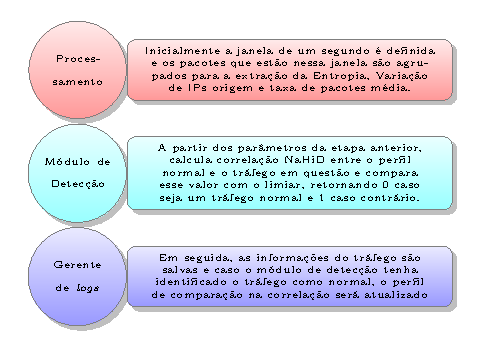
\includegraphics[width=0.8\textwidth]{figs/analiseDarpa.pdf}\\
 	{Fonte: Elaborada pelo autor.}
 	\label{fig:analiseDarpa}
 \end{figure}

.
\subsection{DataMining}
Outra base de dados estudada no trabalho foi a desenvolvida por \cite{DataMining}, a qual consta em sua totalidade por ataques DDoS de quatro tipos:
\begin{itemize}
	\item SIDDoS
	\item HTTP Flood
	\item UDDP Flood
	\item Smurf
\end{itemize}
Esse \textit{dataset} foi gerado em um simulador de rede chamado NS2, um software que representa uma rede de computadores de forma realista. 
A \tabref{Tab:DataMining} mostra os campos do \textit{dataset} avaliado. 

\begin{table}[!b]
	\centering
	\begin{threeparttable}
		\caption{Estrutura base de dados \cite{DataMining}}
		\label{Tab:DataMining}
		%	\small
		\begin{tabular}{c c }
			\toprule
			\textbf{Número} & \textbf{Tempo}
			\\ \midrule
			1 &  Endereço IP origem  \\ \midrule
			2 &  Endereço IP destino  \\ \midrule
			3 &  Id do pacote  \\ \midrule
			4 &  Nó origem  \\ \midrule
			5 &  Nó destino  \\ \midrule
			6 &  Tipo de pacote  \\ \midrule
			7 &  Tamanho do pacote  \\ \midrule
			8 &  Flags  \\ \midrule
			9 &   Id da flag  \\ \midrule
			10 &  Número de sequência  \\ \midrule
			11 &  Número de pacotes  \\ \midrule
			12 &  Número de bytes  \\ \midrule
			13 &  Nome do nó origem  \\ \midrule
			14 &  Nome do nó destino  \\ \midrule
			15 &  Entrada de pacote  \\ \midrule
			16 &  Saída de pacote  \\ \midrule
			17 &  Taxa de pacotes Recebidos \\ \midrule%%%%%%%%%%%%%%%%%%
			18 &  Atraso de nó do pacote  \\ \midrule
			19 &  Taxa de pacotes\\ \midrule
			20 &  Taxa de bytes  \\ \midrule
			21 &  Tamanho  médio do pacote  \\ \midrule
			22 &  Utilização  \\ \midrule
			23 &  Atraso de pacote  \\ \midrule
			24 &  Tempo de envio do pacote  \\ \midrule
			25 &  Tempo de pacote reservado  \\ \midrule
			26 &  Primeiro pacote enviado  \\ \midrule
			27 &  Último pacote reservado \\ \bottomrule
		\end{tabular}
		{Fonte: Elaborada pelo autor, baseada em \cite{DataMining}.}
	\end{threeparttable}
\end{table}

Algumas considerações foram tomadas para a análise dessa base de dados:
\begin{itemize}
	\item Para construir a janela de um segundo, considerou-se a soma de todos os atrasos por pacote:
	\begin{itemize}
	 \item Atraso de nó do pacote.
	 \item  Atraso de pacote.
	 \item Tempo de pacote reservado.
	\end{itemize}
	\item A média das taxas dos pacotes foi considerada dentro da janela de um segundo.
	\item Por ser um \textit{dataset} composto apenas por ataques, a comparação com o limiar inverte-se para denotar o quanto dois pacotes são parecidos na correlação.
\end{itemize}

A base de dados é disponibilizada no formato \textit{Weka Attribute-relation}(extensão arff), o qual é utilizado geralmente para compactar grandes massas de dados e processá-las utilizando técnicas de \textit{machine learning}. Assim, para o processamento dos mesmos as ferramentas Weka e MATLAB foram utilizadas. Inicialmente, no módulo de Pré-Processamento, converteu-se o arquivo .arff para um .mat por meio de \textit{script} e em seguida, com o \textit{dataset} carregado, a janela de um segundo é aplicada, conforme as considerações já mencionadas. Em seguida, os pacotes da janela são agrupados para a extração dos IPs origem, a partir de onde serão calculadas a entropia e  variação, além da taxa de pacotes média. Posteriormente, a partir dos parâmetros da etapa anterior, o módulo de detecção calcula a correlação NaHiD entre o perfil normal e o tráfego em questão e compara com o limiar, retornando 0 caso seja um tráfego normal e 1 caso contrário. Após isso, no gerente \textit{offline}, as informações do tráfego analisado são salvas e caso o módulo de detecção tenha identificado o tráfego como normal, o perfil de comparação na correlação será atualizado.